\documentclass[11pt,twoside]{article}
%\documentclass[10pt,twoside,twocolumn]{article}
\usepackage[english]{babel}
\usepackage{times,subeqnarray}
\usepackage{url}
% following is for pdflatex vs. old(dvi) latex
\newif\myifpdf
\ifx\pdfoutput\undefined
%  \pdffalse           % we are not running PDFLaTeX
   \usepackage[dvips]{graphicx}
\else
   \pdfoutput=1        % we are running PDFLaTeX
%  \pdftrue
   \usepackage[pdftex]{graphicx}
\fi
\usepackage{apatitlepages}
% if you want to be more fully apa-style for submission, then use this
%\usepackage{setspace,psypub,ulem}
%\usepackage{setspace} % must come before psypub
%\usepackage{psypub}
%\usepackage{psydraft}
\usepackage{one-in-margins}  % use instead of psydraft for one-in-margs
\usepackage{scicite}
%\usepackage{apa}       % apa must come last
% using latex2e as standard, use the following for latex209
% \documentstyle [times,11pt,twoside,subeqnarray,psydraft,apa,epsf]{article}
\input netsym

% tell pdflatex to prefer .pdf files over .png files!!
\myifpdf
  \DeclareGraphicsExtensions{.pdf,.eps,.png,.jpg,.mps,.tif}
\fi

\newenvironment{sciabstract}{%
\begin{quote} \bf}
{\end{quote}}

\renewcommand\refname{References and Notes}

\newcounter{lastnote}
\newenvironment{scilastnote}{%
\setcounter{lastnote}{\value{enumiv}}%
\addtocounter{lastnote}{+1}%
\begin{list}%
{\arabic{lastnote}.}
{\setlength{\leftmargin}{.22in}}
{\setlength{\labelsep}{.5em}}}
{\end{list}}

% use 0 for psypub format 
\parskip 2pt
% for double-spacing, determines spacing 
%\doublespacing
%\setstretch{1.7}

\columnsep .25in   % 3/8 in column separation

\def\myheading{ Deep Predictive Learning }

% no twoside for pure apa style, use \markright with heading only
\pagestyle{myheadings}
\markboth{\hspace{.5in} \myheading \hfill}{\hfill O'Reilly, Russin, \& Rohrlich \hspace{.5in}}

\bibliographystyle{Science}

\title{ Deep Predictive Learning as a Model of Human Learning } 

\author{Randall C. O'Reilly, Jacob L. Russin, and John Rohrlich\\
  Departments of Psychology and Computer Science\\
  Center for Neuroscience\\
  University of California, Davis \\
  1544 Newton Ct\\
  Davis, CA 95616\\
  {\small oreilly@ucdavis.edu}\\}

\def\mynote{Draft Manuscript: Do not cite or quote without
  permission.\\

  R. C. O'Reilly is Chief Scientist at eCortex, Inc., which may derive indirect benefit from the work presented here.

  Supported by: ONR grants N00014-18-1-2116 (Deep learn), N00014-14-1-0670 / N00014-16-1-2128 (Bidir vis), N00014-18-C-2067 (MDM)

  This work utilized the Janus supercomputer, which is supported by the National Science Foundation (award number CNS-0821794) and the University of Colorado Boulder. The Janus supercomputer is a joint effort of the University of Colorado Boulder, the University of Colorado Denver and the National Center for Atmospheric Research.
}


\begin{document}

% sloppy is the way to go!
\sloppy
\raggedbottom
\baselineskip20pt

\maketitle 

\clearpage

\begin{sciabstract}
  Now that's abstract..
\end{sciabstract}

\clearpage

\pagestyle{myheadings}

The success of deep convolutional neural networks (DCCN's) \cite{KrizhevskySutskeverHinton12,LeCunBengioHinton15,Schmidhuber15a} in object recognition and many other domains raises the question of how well they model human learning, at both neural and cognitive levels.  Although the engine of these models, error backpropagation \cite{RumelhartHintonWilliams86}, has long been questioned on biological grounds \cite{Crick89}, many biologically-plausible mechanisms have been proposed \cite{OReilly96,XieSeung03,BengioMesnardFischerEtAl17}.  However, the need for massive amounts of labeled data still makes these models cognitively implausible: non-human primates and infants learn to recognize and categorize objects without massive amounts of labeled data.  An alternative, biologically-plausible approach is to use {\em predictive error-driven learning}, where error signals arise from differences between a prediction of what will happen next, and what actually does happen \cite{Elman90,ElmanBatesKarmiloff-SmithEtAl96}.  All this requires, in principle, is events to unfold over time, and a learning system that is somehow organized to generate predictions of these events.  Furthermore, the ability to accurately predict complex real-world events would imply that considerable knowledge has been absorbed in the process of so doing, and thus there is a reason to believe that predictive learning could power sophisticated, important forms of developmental learning.

Here we show that circuits between the neocortex and thalamus, replicated across the extent of these structures, have several distinctive properties that directly support predictive error-driven learning. Furthermore, when implemented in a computational model employing a biologically-plausible form of error backpropagation \cite{OReilly96,OReillyMunakata00,OReillyMunakataFrankEtAl12}, along with several other important properties of the mammalian visual system, the model learns to systematically categorize 3D objects according to invariant shape properties, in a way that matches human judgments of these same objects, and is consistent with neural representations in inferotemporal (IT) cortex in primates.  Comparison models with the same structure but using standard non-biological error-backpropagation learning, and models using the state-of-the-art {\em PredNet} predictive learning architecture \cite{LotterKreimanCox16}, support the importance of predictive learning for more strongly shaping internal representations, but these models do not learn much beyond the similarities present at the lowest visual levels.  Thus, we argue that incorporating biological properties of the brain can potentially provide a better understanding of human learning at multiple levels relative to existing DCCN models.

\begin{figure}
  \centering\includegraphics[width=6in]{figs/fig_deepleabra_wwi_abc_pred_model_frames}
  \caption{\small {\bf a)} Schematic illustration of the temporal evolution of information flow in the DeepLeabra model predicting visual sequences, over two alpha cycles of 100 msec each.  During each alpha cycle, the V2 Deep layer uses the prior 100 msec of context information to generate a prediction or expectation (minus phase) over the pulvinar thalamic relay cell (TRC) neurons, of what will happen next.  The bottom-up actual outcome is driven over the pulvinar via the 5IB strong driver inputs from V1, providing the {\em plus} or {\em target} phase of learning.  Error-driven learning occurs as a function of the {\em temporal difference} between the plus and minus activation states, in both superficial and deep networks, via the pulvinar projections into these networks.  The 5IB bursting in V2 drives an update of the local temporal context information in V2 Deep layers, which is used in generating the minus phase prediction in the next alpha cycle, and so on.  These same 5IB cells drive a plus phase in higher area TRC's as well, which perform the same kind of {\em local} predictive auto-encoder learning as shown for V2 here.  {\bf b)} The three-visual-stream deep predictive learning model ({\em What-Where-Integration, WWI} model). The dorsal {\em Where} pathway learns first, using easily-abstracted {\em spatial blobs}, to predict where an object will move next, based on prior motion history, visual motion, and saccade efferent copy signals.  This drives strong top-down inputs to lower areas with accurate spatial predictions, leaving the {\em residual} error concentrated on {\em What} and {\em What * Where} integration information.  The V3 and DP (dorsal prelunate) areas constitute the {\em What * Where} integration pathway, helping bind features and locations.  V4, TEO, and TE are the {\em What} pathway, learning abstracted object category representations, which also drive strong top-down inputs to lower areas.  {\em s} suffix = superficial layer, {\em d} = deep layer, and {\em p} = pulvinar.  {\bf c)} An example sequence of 8 frames that the model learned to predict, with the reconstruction of each image based on the V1 gabor filters ({\em V1 recon}), and a reconstruction of the model-generated prediction for each frame over the higher resolution V1hp pulvinar layer.  The relatively low resolution encoding of the image makes these somewhat difficult to interpret, but this and other examples in the supplemental material, along with the prediction correlation values as shown, all indicate that the model has learned somewhat vague but broadly accurate predictions.  The eye icons indicate when a saccade occurred.}
  \label{fig.model}
\end{figure}

Motivated by biological evidence, we hypothesize that sensory predictions in posterior neocortex are generated roughly every 100 msec (i.e., the {\em alpha} rhythm, 10 Hz), by neurons in the deep layers of the neocortex that project to the pulvinar nucleus of the thalamus (Figure~\ref{fig.model}a).  The pulvinar represents this top-down prediction for roughly 75 msec of the alpha cycle as it develops, after which point the layer 5IB intrinsic-bursting neurons send strong, bottom-up driving input to the pulvinar, representing the actual sensory stimulus \cite{ShermanGuillery06}.  These 5IB neurons burst at the alpha frequency, determining the overall timing of the predictive learning cycle, along with other dynamic parameters of the thalamocortical circuit \cite{LorinczKekesiJuhaszEtAl09,FranceschettiGuatteoPanzicaEtAl95,SaalmannPinskWangEtAl12}.  Consistent with the temporal-difference nature of biologically-plausible error signals in this framework, the prediction error is implicit in the temporal difference between these two periods of activity within the alpha cycle over the pulvinar.  The pulvinar sends broad projections back up to all of the areas that drive top-down predictions into it \cite{Shipp03,Mumford91}, thus broadcasting this error signal to drive local synaptic plasticity in the neocortex. This is mathematically equivalent to performing gradient descent to minimize overall prediction errors.  This computational framework makes sense of otherwise puzzling anatomical and physiological properties of the cortical and thalamic networks \cite{ShermanGuillery06}, and is consistent with a wide range of detailed neural and behavioral data regarding the effects of the alpha rhythm on learning and perception \cite{BuffaloFriesLandmanEtAl11,VanRullenKoch03,JensenBonnefondVanRullen12,FiebelkornKastner19}.  It has many testable differences from other existing forms of predictive learning that have been proposed over the years, at varying levels of biological detail \cite{Mumford92,RaoBallard99,KawatoHayakawaInui93,Friston05}.

A critical question for predictive learning is whether it can develop higher-level, more abstract ways of representing sensory inputs, that go beyond the raw low-level structure of these inputs, while learning from nothing other than predicting these raw visual inputs.  For example, can predictive learning really replace the labor-intensive process of generating human-labeled image datasets where abstract category information is explicitly used to train object recognition models via error-backpropagation?  From a cognitive perspective, there is considerable evidence that non-verbal primates, and pre-verbal human infants, naturally develop abstract categorical encodings of visual objects in IT cortex \cite{CadieuHongYaminsEtAl14}, without relying on any explicit external categorical labels.  Existing predictive-learning models based on error backpropagation \cite{LotterKreimanCox16} have not demonstrated this result; instead, these models are typically tested on their ability to subsequently train using the human-generated labels, but there are many ways in which prior training could facilitate such training without fully forming systematic categories de-novo.

To determine if our biologically-based predictive learning model can naturally form such categorical encodings in the complete absence of externally-provided category labels, we showed the model brief movies of 176 specific 3D object exemplars drawn from 20 different categories selected from the CU3D-100 dataset \cite{OReillyWyatteHerdEtAl13}.  The objects moved and rotated in 3D space over 8 movie frames, where each frame was sampled at the 10 Hz alpha frequency.  There were also saccadic eye movements every other frame, with an efferent copy signal to enable full prediction of the effects of the eye movement, which allows the model to capture predictive remapping (a widely-studied signature of predictive learning in the brain) \cite{DuhamelColbyGoldberg92,CavanaghHuntAfrazEtAl10}, and introduces further predictive-learning challenge.  The only learning signal available to the model was the temporal difference prediction error between what it predicted to see in the next frame, compared to what was actually seen.  

\begin{figure}
  \centering\includegraphics[width=6in]{fig_rsa_leabra_expt1}
  \caption{\small {\bf a)} Category similarity structure that developed in the highest layer, TE, of the biologically-based predictive learning model, showing 1-correlation similarity of the TE representation for each object against every other object. Blue cells have high similarity, and model has learned block-diagonal clusters or categories of high-similarity groupings, organized according to overall object shape as identified via agglomerative clustering and similarity matrix plotting, see supplemental materials. {\bf b)} Human similarity ratings for the same objects, where each cell is 1 - proportion of time the given pair of objects were rated as more similar than another pair of objects (see supplemental material for details of the experiment).  The resulting similarity matrix generally exhibits the same categorical structure as the model (confirmed by agglomorative cluster analysis).  {\bf c)} Emergence of abstract category structure over the hierarchy of layers.  Red line shows correlation similarity between the similarity matrix for TE (shown in panel a) against the similarity matrix computed for every other layer, and the black line shows the correlation similarity for the V1 layer matrix against every other layer (1 = identical; 0 = orthogonal). Both show that IT layers (TEO, TE) progressively differentiate from raw input similarity structure present in V1.}
  \label{fig.rsa}
\end{figure}

We performed a representational similarity analysis (RSA) on the learned activity patterns at each layer in the model, and found that the highest IT layer (TE) produced a systematic organization of the 3D objects into 5 different categories (Figure~\ref{fig.rsa}a), which visually correspond to the overall shape of the objects (pyramid-shaped, vertically-elongated, round, boxy / square, and horizontally-elongated). This organization of the objects matches that produced by humans making shape similarity judgments on the same set of objects (Figure~\ref{fig.rsa}b; see supplemental material for methods and further analysis).  Critically, Figure~\ref{fig.rsa}c shows that the overall similarity structure present in IT layers (TEO, TE) of the biological model is significantly different from the similarity structure at the level of the V1 primary visual input layer of the model.  Thus, the model has learned an abstract way of organizing these objects that goes beyond the raw pixel-level information, despite only being trained to generate accurate predictions about what the scene will look like next, at the level of this low-level visual representation.  Furthermore, this abstract category organization reflects the overall visual shapes of the objects as judged by human participants looking at the same objects, suggesting that the model is learning about the same kind of overall geometrical shape information that is apparent once these objects are encoded in an invariant way that abstracts across the motion, rotation, and scaling transformations present in the V1 visual inputs.  We further verified that at the highest IT levels in the model, a consistent representation is present across different views of the same object (supplementary Figure X), and, as shown in Figure~\ref{fig.rsa}a, across multiple objects within the same category (the dark blue cells there reflect close similarity across different objects).

\begin{figure}
  \centering\includegraphics[width=4in]{fig_rsa_leabra_macaque}
  \caption{\small Comparison of progression from V4 to IT in macaque monkey visual cortex (top row, from Cadieu et al, 2014) versus same progression in model (replotted using comparable color scale).  Although the underlying categories are different, and the monkeys have a much richer multi-modal experience of the world that could help reinforce categories such as foods and faces, our model nevertheless shows a similar qualitative progression in extent of stronger categorical structure in IT, where the block-diagonal highly similar representations are more consistent across categories, and the off-diagonal differences are stronger and more consistent as well (i.e., categories are also more clearly differentiated).  Note that the critical difference in our model versus those compared in Cadieu et al 2014 and related papers is that they explicitly trained their models on category labels, whereas our model is {\em entirely self-organizing} and has no external categorical training signal.}
  \label{fig.macaque}
\end{figure}

Further evidence for the progressive nature of representation development in our model is shown in Figure~\ref{fig.macaque}, which compares the similarity structures in layers V4 and IT in macaque monkeys \cite{CadieuHongYaminsEtAl14} with those in corresponding layers in our model.  In both the monkeys and our model, the higher IT layer builds upon and clarifies the noisier struture that is emerging in the earlier V4 layer.  Considerable other work has also compared DCNN representations with these same data from monkeys \cite{CadieuHongYaminsEtAl14}, but it is essential to appreciate that those DCNN models were explicitly trained on the category labels, making it somewhat less than surprising that such categorical representations developed.  By contrast, we reiterate that our model has discovered its categorical representations entirely on its own, with no explicit categorical inputs or training of any kind.


Fig 3a: Category similarity structure in the highest IT layer (TE) of the backpropagation model, which is essentially binary in structure.  Some “ground truth” object categories (e.g., piano, slr camera) are split across these two categories, as evidenced by the transition not taking place cleanly along the black horizontal and vertical dividing lines (which split along the “ground truth” categories).  Representations here are overall much more similar to each other — colorscale is renormalized to use full color range compared to equivalent 2a figure.
3b: Comparison of V1 RSA similarity structure across layers, for backpropagation model (red line) compared to data previously shown in 2d for biological model (black line). Unlike the biological model, the V1-level structure persists largely intact throughout the backprop model, except in layer V3s which is most directly influenced by spatial prediction errors.  Thus, there is no evidence that the backpropagation model has developed significantly different structure beyond that present in the lowest V1 levels.
3c: Comparison of TE RSA similarity structure across layers, for all combinations of backpropagation vs. biological model (black line is same as 2d).  The red line shows that, consistent with 3b, the TE-level structure in backprop is consistent with most layers except V3, again indicating a lack of significant novel structure in TE.  The blue line shows that the TE structure in the biological model (2a) is not a good fit for any layers in the backprop model, and the green line shows that IT (TEO, TE) layers of the biological model strongly diverge from the backprop TE representations.

Figure 3 shows the results from a non-biological backpropagation-based version of the same model architecture.  In this model, the highest layers in the network form a more degenerate binary category structure overall, and the detailed item-level similarity structure does not diverge significantly from that present at the lowest V1 inputs, indicating that it has not formed novel systematic structured representations, in contrast to those formed in the biologically-based model.  Thus, it is clear that the additional biologically-motivated properties of the original model are playing a critical role in the development of abstract categorical representations. These properties include: excitatory bidirectional connections, inhibitory competition, and a Hebbian form of learning that serves as a regularizer in addition to the predictive error-driven learning \cite{OReilly98,OReillyMunakata00}.  Ongoing work is attempting to determine which of these is essential, perhaps all of them, by introducing some of these properties into the backpropagation model, though this is difficult because full bidirectional recurrent activity propagation, which is essential for conveying error signals top-down in the biological network, is incompatible with the standard efficient form of error backpropagation, and requires much more computationally intensive and unstable forms of fully recurrent backpropagation (Williams et al, etc).  Furthermore, Hebbian learning requires inhibitory competition which is difficult to incorporate within the backpropagation framework — results shown next demonstrate the importance of this Hebbian learning factor within the biological model.


Fig 4a: contributions of the dorsal “where” pathway in the biological model, including LIP (lateral inferior parietal sulcus area), V3, and DP (dorsal prelunate).  Lesioning this pathway causes the IT (TEO, TE) representations to be much more similar to those in V1, and, likewise, the TE representations to be relatively similar to those throughout the network.  Thus, having the spatial pathway regress out the spatial component of prediction error is essential for concentrating the residual error on object features, which are learned by the ventral “what” pathway into IT.  b) shows that the what / where organization is also important in the backprop version of the model — what little organization it developed that diverged from V1 is eliminated when the dorsal where pathway is fully lesioned.  Furthermore, when trained as a pure auto-encoder of the current image (instead of predicting the next), it fails to develop anything other than a pure V1-level surface representation.
4b: hebbian param diff — easily has big effects, key for connecting to bio stuff.

Despite these difficulties, the biological model results were based on extensive experimentation and theorizing about several other specific properties that should be important for enabling it to learn these abstract categorical representations, and we are able to directly test the relevance of many of these factors.  For example, we hypothesized that separating the overall prediction problem between spatial ``where'' vs. non-spatial ``what'' pathways, a well-established property of the dorsal vs. ventral streams of the visual system \cite{UngerleiderMishkin82}, would be essential for partitioning the overall prediction error.  The spatial where pathway can learn relatively quickly to predict the overall spatial trajectory of the object (and anticipate the effects of saccades), and thus effectively regress out that component of the overall prediction error, leaving the residual error concentrated in object feature information, which can train the ventral “what” pathway to develop abstract visual categories.  Figure 4a shows that, indeed, when the where pathway is lesioned to varying degrees, it systematically impairs the formation of the abstract categorical representations in the intact what pathway.  Figure 4b shows the same manipulation on the backpropagation model, with similar results: what little deviation it exhibited from the pure V1 similarity structure is eliminated with a complete dorsal pathway lesion.  In both models, lesioning the dorsal where pathway significantly impacted overall prediction error, as would be expected (Supplemental Figure X).  Regarding the other biological properties, Figure 4c shows the impact of changing Hebbian learning parameters, reducing the strength of lateral context connections within the IT pathway, and eliminating the temporally-delayed nature of these connections, all of which significantly impaired the formation of categorical representations.  The effects of other tests are reported in the supplemental material.

A final experiment tested the importance of performing predictive learning, as compared to an auto-encoder, which learned to encode and reproduce the visual inputs within a single frame, as compared to having to predict the next frame from the current one.  Auto-encoders are closely related to predictive learning models, and have been widely explored (cites).  However, the encoder paradigm is more susceptible to degenerate solutions amounting to performing a “mindless copy” as opposed to a “deep encoding”, and considerable effort must be made to discourage such solutions, whereas prediction, being “about the future”, is not susceptible to these solutions (except in fully static environments where the two approaches converge).  We tested an auto-encoder version of the backpropagation model which reproduced the current input frame, instead of trying to predict the next frame in the movie, and found that this completely eliminated any development of non-V1 similarity structure in the model (Figure 4b).

In conclusion, we have demonstrated that learning based strictly on predicting what will be seen next is, in conjunction with a number of critical biologically-motivated network properties and mechanisms, capable of generating abstract, invariant categorical representations of the overall shapes of objects, with a structure that matches human shape similarity judgments.  Thus, we have demonstrated that predictive learning has the potential to go beyond the surface structure of its inputs, and develop systematic, abstract encodings of the “deeper” structure of the environment.  Considerable further work remains to be done to more precisely characterize the essential properties of our biologically-motivated model necessary to produce this abstract form of learning, and to further explore the full scope of abstract learning across different domains.  We strongly suspect that extensive cross-modal predictive learning in real-world environments is a significant factor in human and specifically infant development and could greatly multiply the opportunities for the formation of higher-order abstract representations that more compactly and systematically capture the structure of the world.  Furthermore, extending predictive learning to encompass motor interactions with the environment can potentially create much richer opportunities for deeper learning.  Future versions of these models could thus potentially answer the question of how deep an understanding a pre-verbal human, or a non-verbal primate, can extract from its environment through such predictive learning mechanisms.  This would then represent the foundation upon which language and cultural learning builds, to shape the full extent of human intelligence.

\bibliography{ccnlab}

\end{document}
